\documentclass[11pt,final] {article}
\usepackage[margin=0.5in,landscape]{geometry}
\usepackage{setspace}
\usepackage{amsmath}
\usepackage{sidecap}
\usepackage{fancyhdr}
\usepackage{float}
\usepackage{graphicx}

\pagestyle{fancy}
\renewcommand{\headrulewidth}{0pt}
\fancyhead{}
\fancyfoot{}

\graphicspath{{./}}

\begin{document}

\begin{center}
{\bfseries \Huge Making Espresso}
\end{center}

~\\

\begin{tabular}{p{1in} p{3in} p{0.5in} p{1in} p{3in}}
	\raisebox{-0.9in}{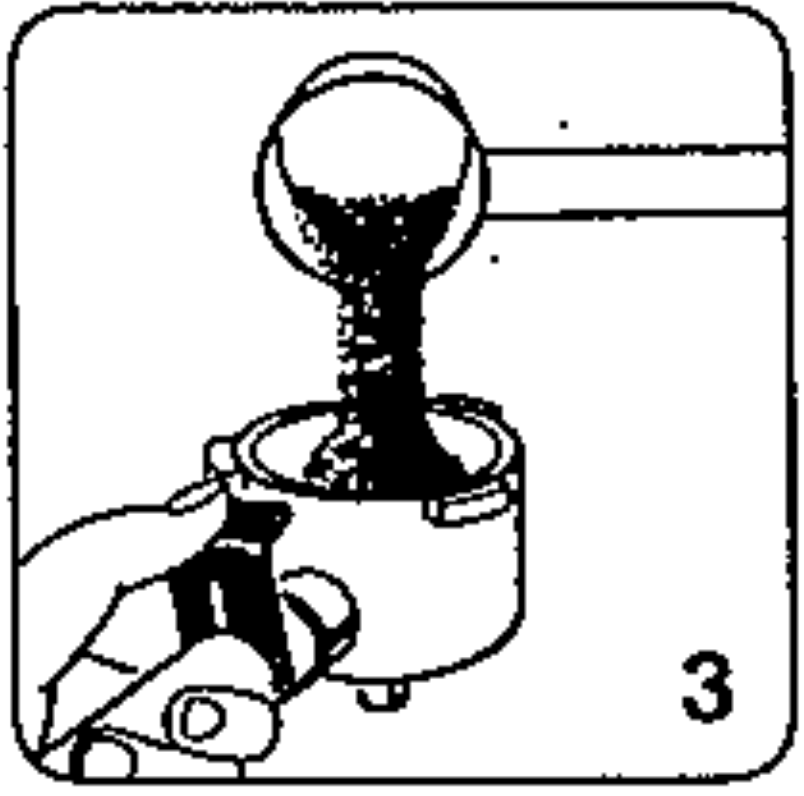
\includegraphics[width=1in]{01}} & Add coffee grounds to the filter holder. (People who science tell us that a medium-fine ground will give you the best results!) & &\raisebox{-0.9in}{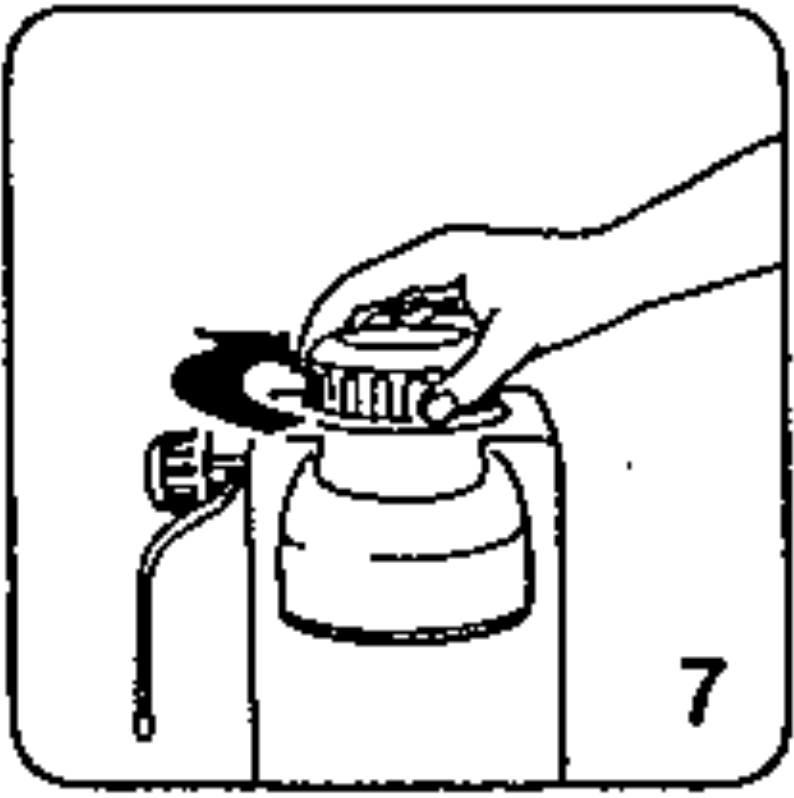
\includegraphics[width=1in]{05}} & Screw the lid on tightly \\
	
	~\\
	
	\raisebox{-0.9in}{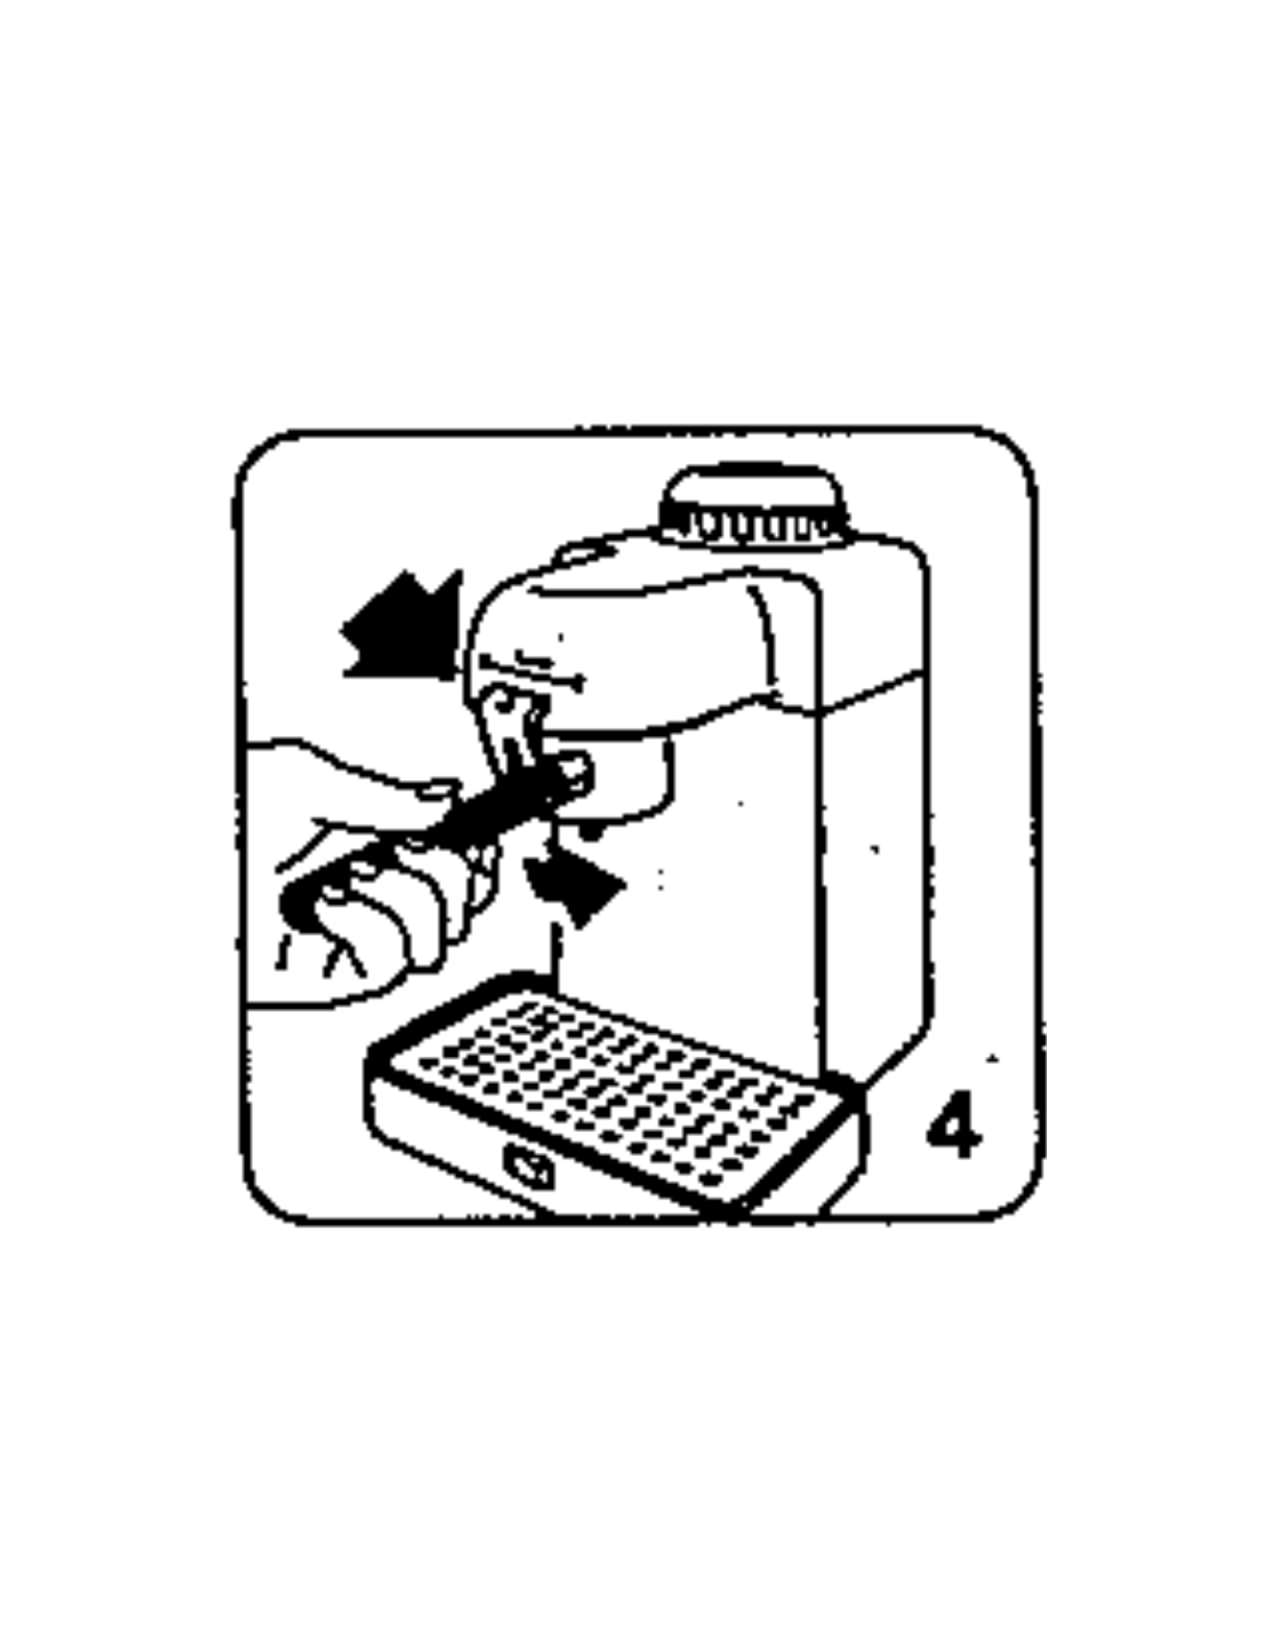
\includegraphics[width=1in]{02}} & Attach the filter holder to the espresso machine and twist fully to the right to lock into place. & &\raisebox{-0.9in}{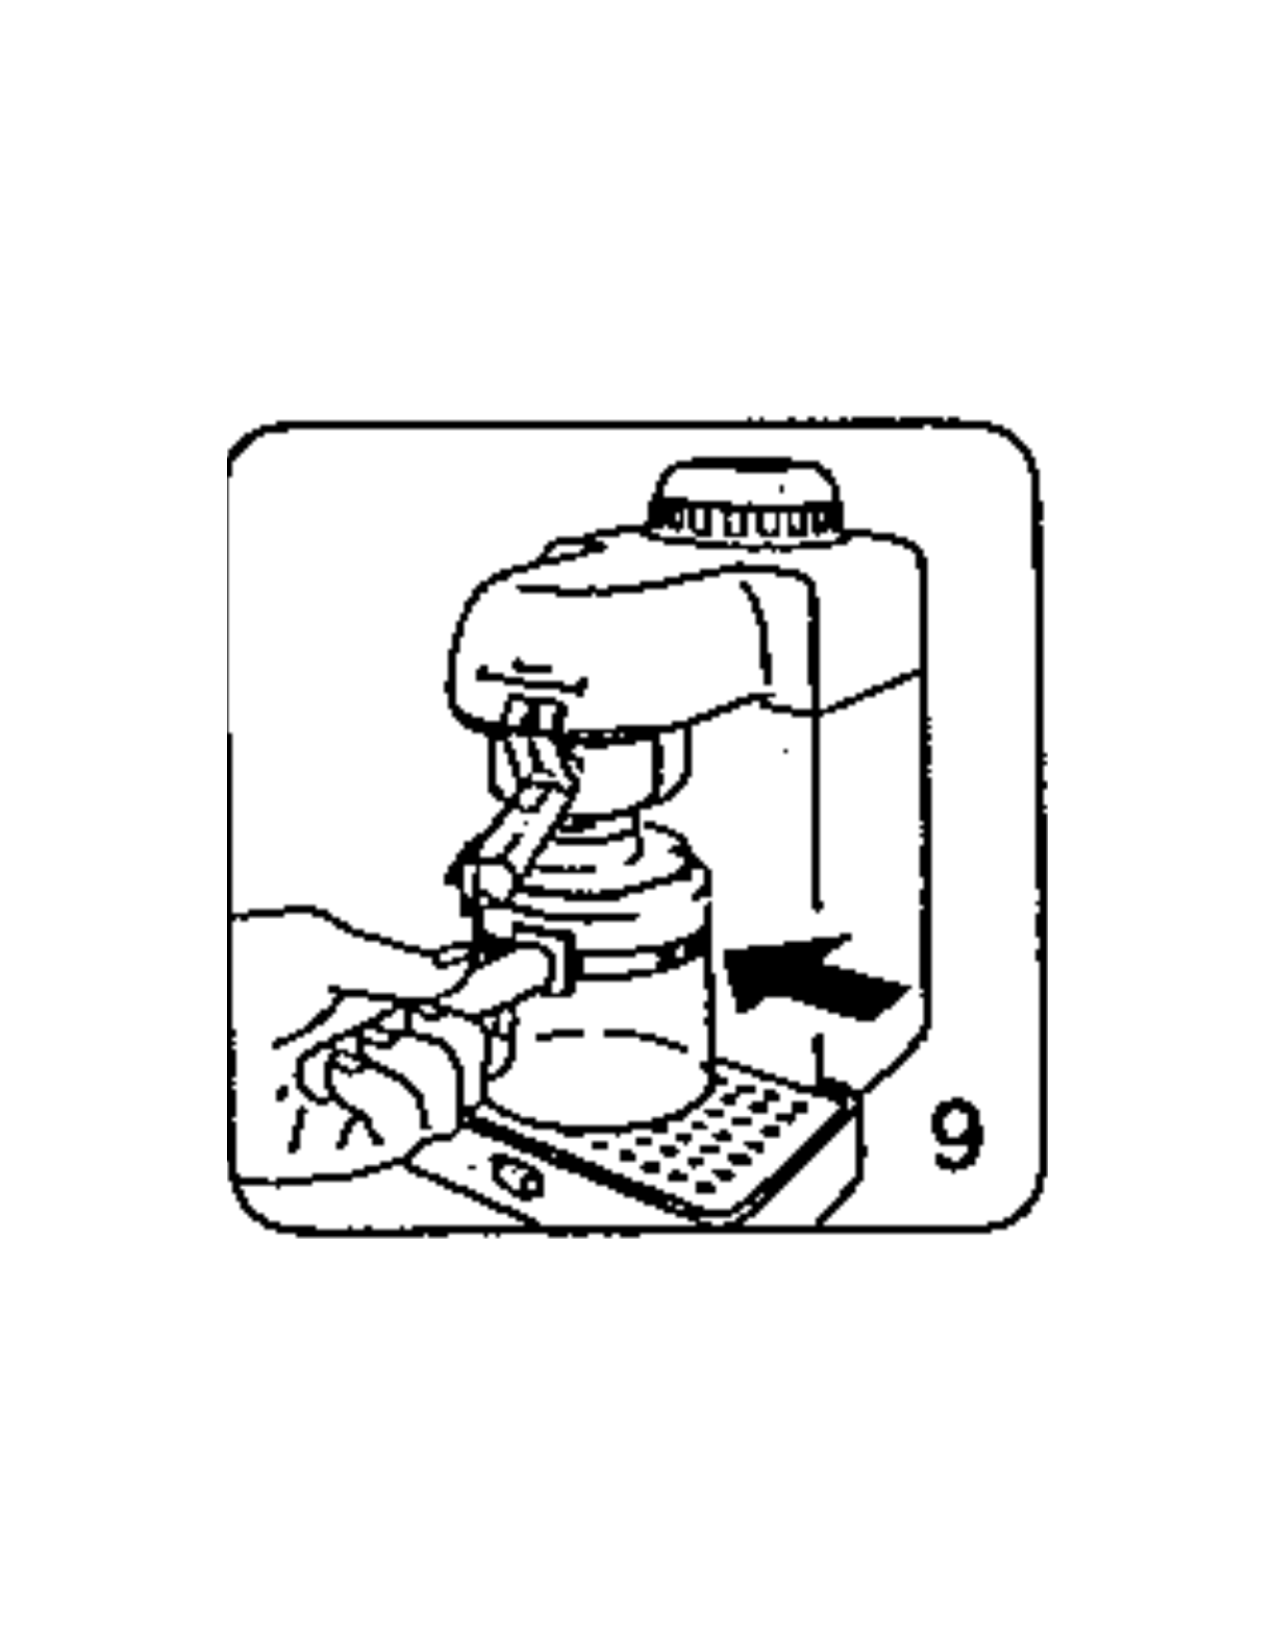
\includegraphics[width=1in]{06}} & Place the carafe or your coffee mug on the overflow grid.\\

	~\\
		
	\raisebox{-0.9in}{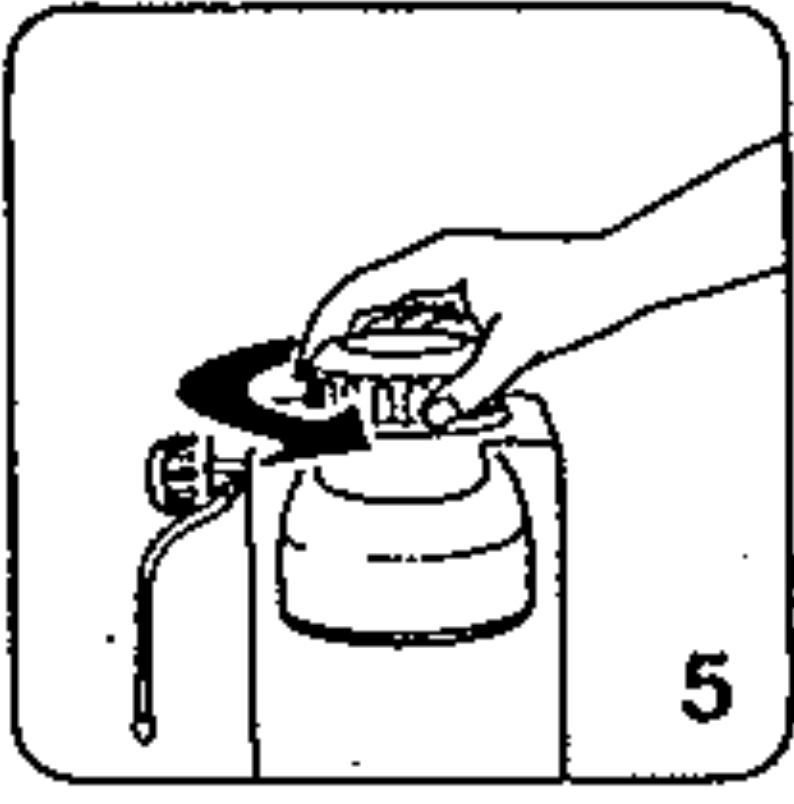
\includegraphics[width=1in]{03}} & Unscrew the cap. & &\raisebox{-0.9in}{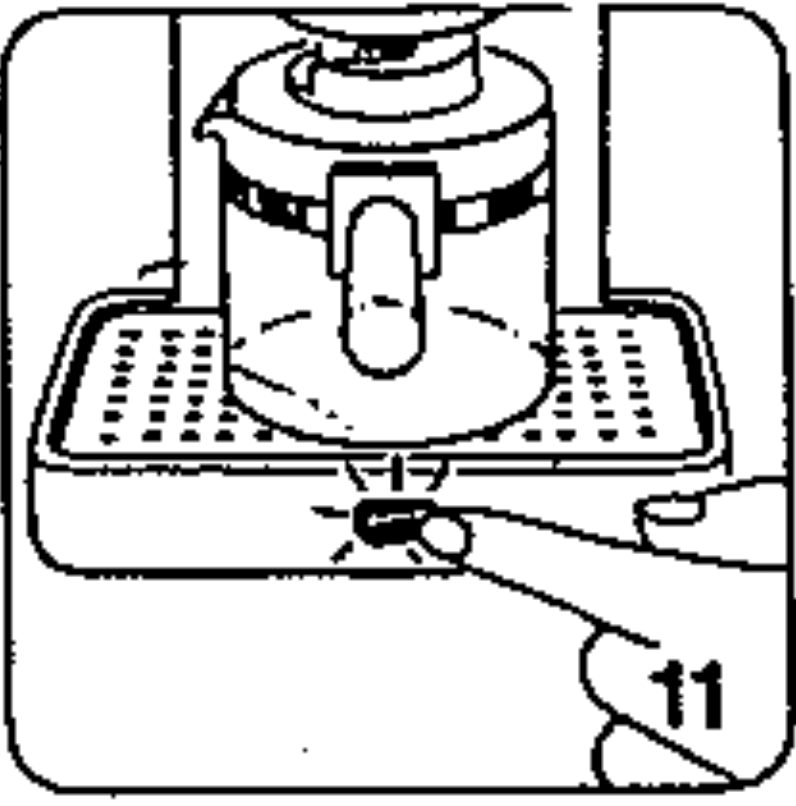
\includegraphics[width=1in]{07}} & Turn it on! You can nearly taste the caffeine already! (It'll take about $1.5$ to $2$ minutes for the water to reach the proper temperature.\\

	~\\
		
	\raisebox{-0.9in}{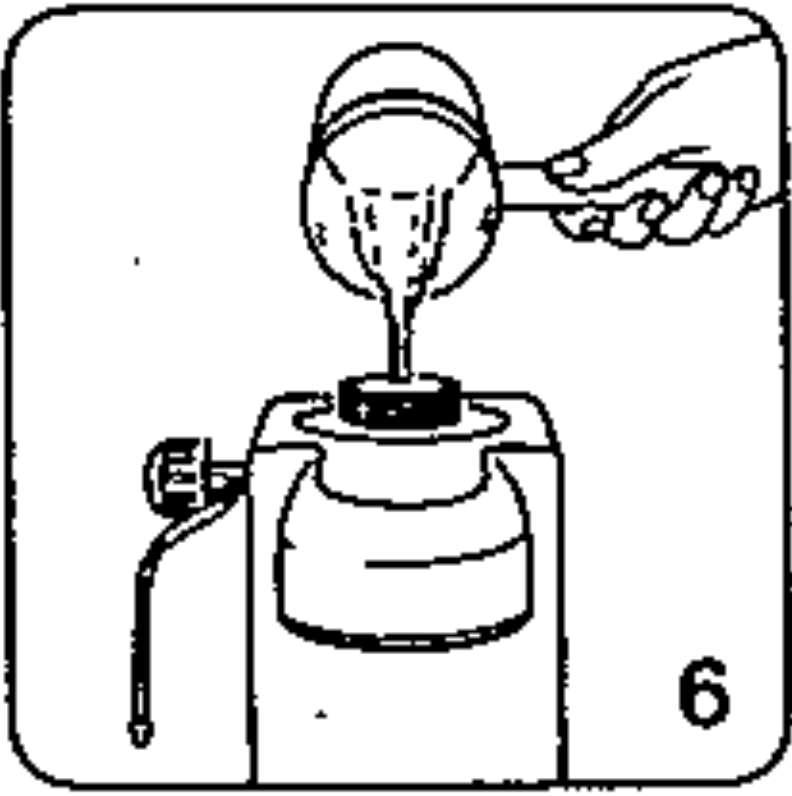
\includegraphics[width=1in]{04}} & Add water measured using the glass carafe (don't fill with water above the top line marked `4').& &\raisebox{-0.9in}{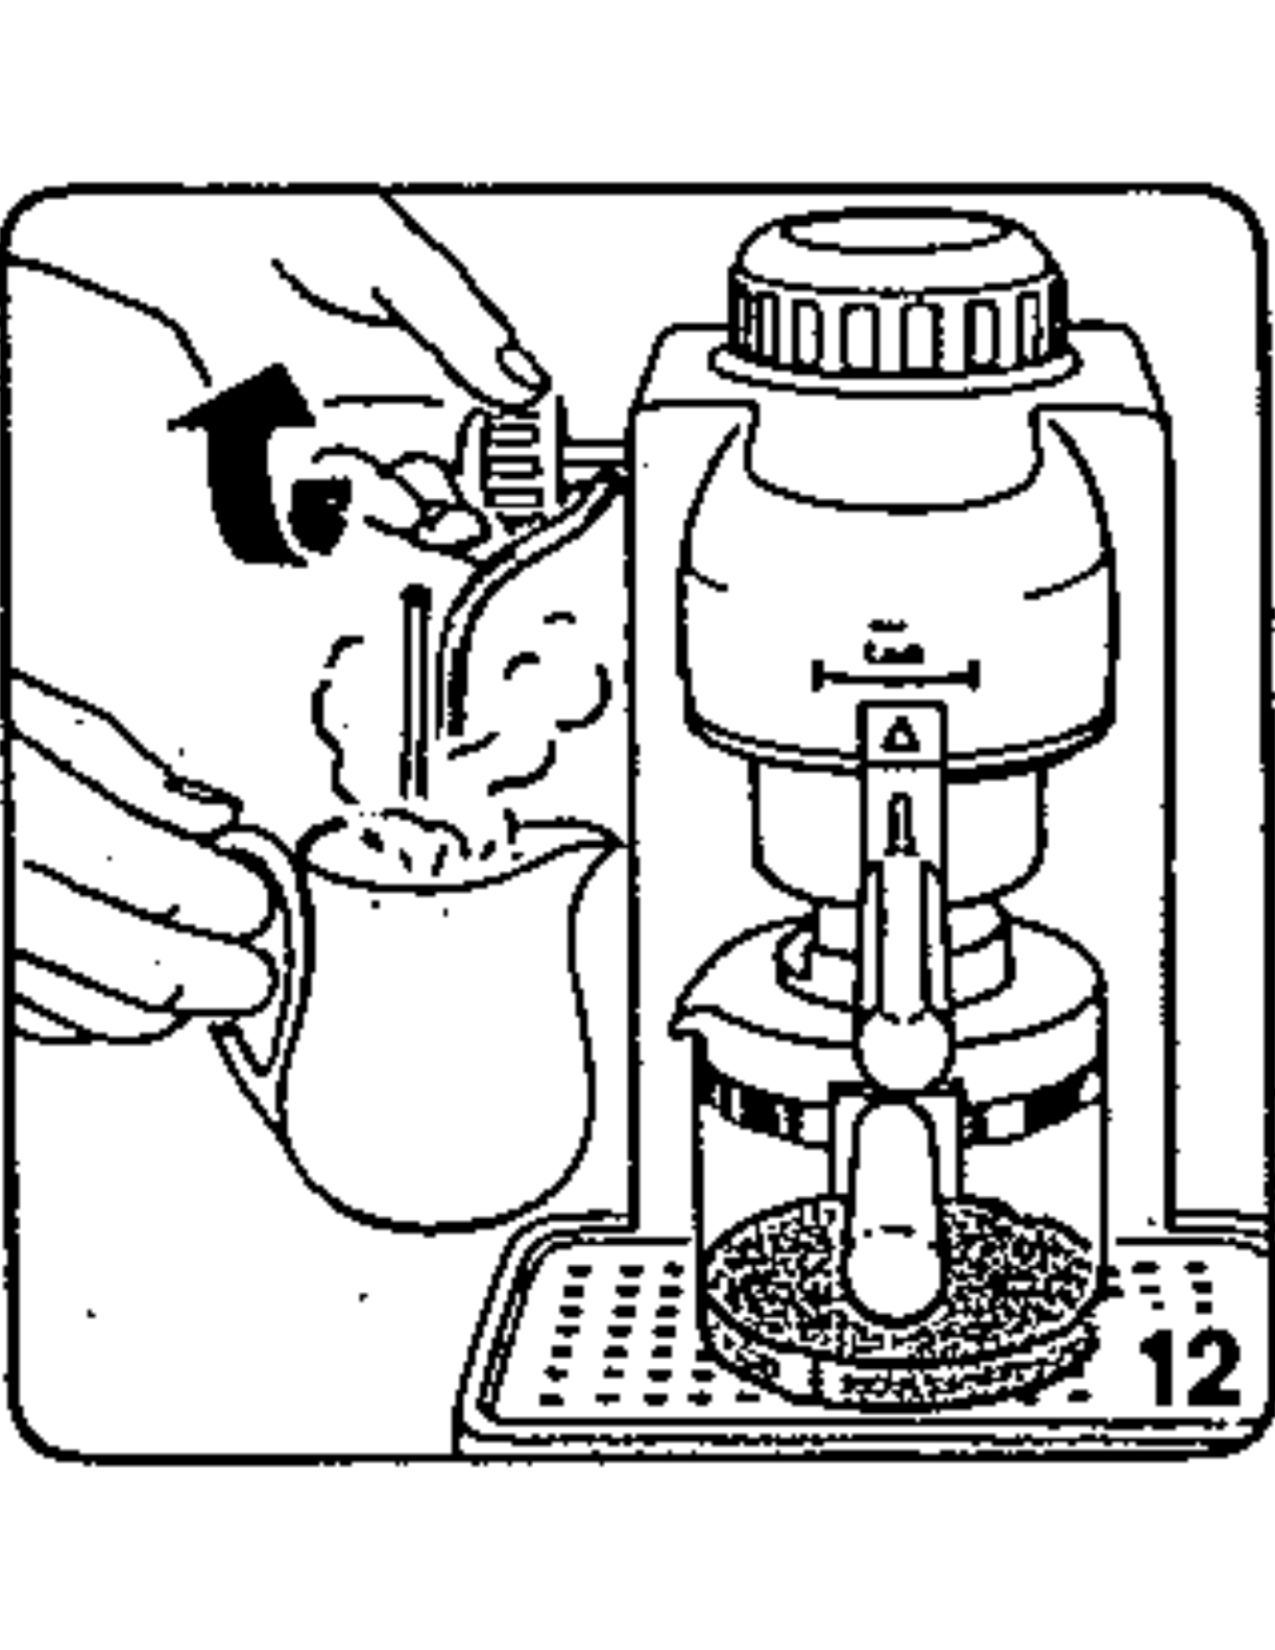
\includegraphics[width=1in]{08}} & Once espresso begins to flow, you can also steam milk to make a cappuccino. Fill a small pitcher about 1/3 with milk. Open the steam nozzle just above the surface of the milk and slowly lower it beneath the surface. (The black rubber nib should be 3/4 submerged.) Remove the pitcher and close the nozzle.\\

\end{tabular}\\[0.5cm]

\begin{center}
{\bfseries \Large Remember to turn off the machine once you're done!}\\

If you used the steam wand, please clean it thoroughly with a damp paper towel or rag to prevent\\ milk buildup that can clog the steam wand and ruin your delicious, delicious cappuccino. Cause that's just bad times for everyone.
\end{center}
\end{document}